
\chapter{Models}
	\section{Successive modeling phases}
		
		\begin{wrapfigure}[18]{l}{4cm}
		\vspace{-5mm}	
		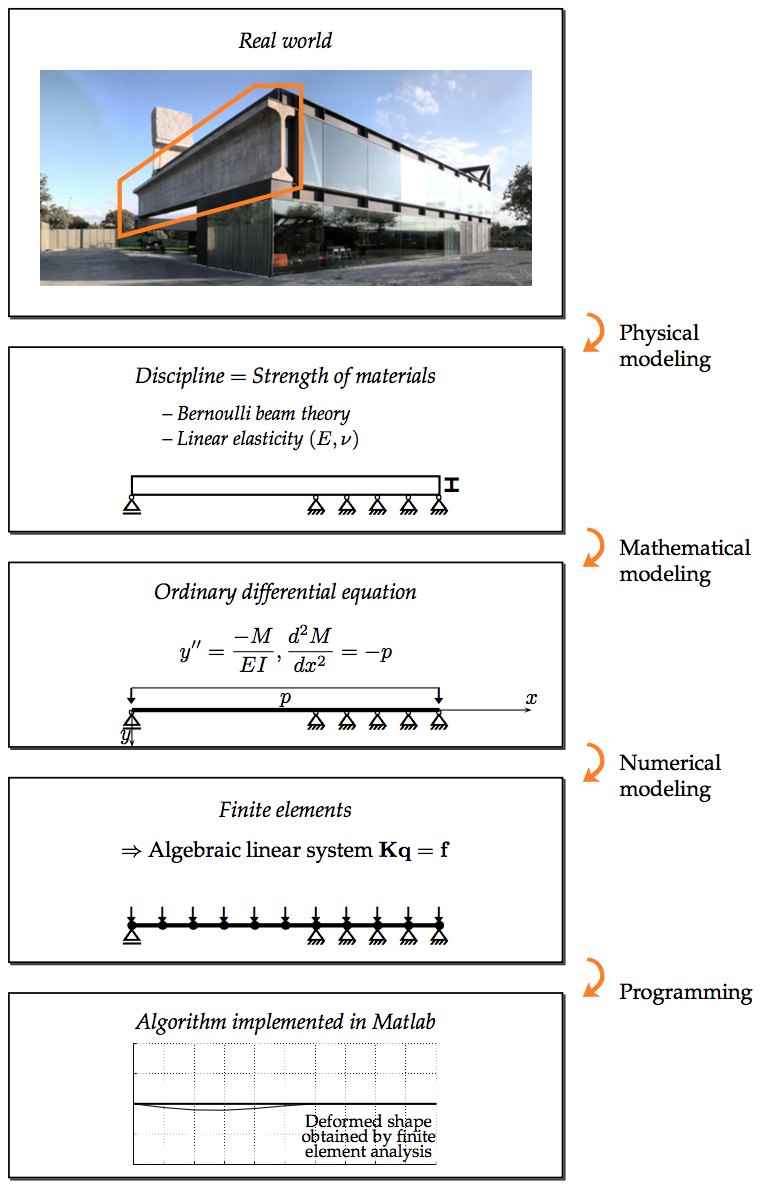
\includegraphics[scale=0.35]{ch2/1}
		\captionof{figure}{}
		\end{wrapfigure}		
		To implement a model on the computer we need:		
		\begin{itemize}
				\item[•] a \textbf{physical model:} step of defining the disciplines involved and (e.g. fluid dynamics) and the hypothesis regarding the material law (e.g. elasticity); In our example we can see a building where there is a huge beam. We want to model this and first this is a volume. We will represent it in 2D and the first question is "do I have shear stress". Yes there is a wall below leading to the small triangles on the figure, assuming that there is no displacement in y axis. Then the second question is "do I care of elastic behavior of concrete or is linear elasticity enough?" $\rightarrow$ assumption. 
				
			\ 	\item[•] a \textbf{mathematical model:} translation of the physical principles into mathematical language; In the example we have the relation with $y''$ and the one concerning the load, which is the roof part. We are assuming here that the weight of the roof is equally distributed. 
				\end{itemize}
				\ \\
				\begin{itemize}
				\item[•] a \textbf{numerical model:} implementing an algorithm able to solve the previous point equations; 
				What we do is in fact cutting our element in several elements, separated by nodes. The distributed forces will then be applied on that nodes. \textbf{THE} equation for finite element is: $Kq = f$ where $K$ is a 6x6 matrix and represents \textbf{stiffness}, q \textbf{displacement} and f \textbf{force} are 6x1 vectors. 
				
			\	\item[•] a \textbf{computer model:} implementation of an in-house code or a commercial software product, based on the previous point. \\
				In this course we will be using a displacement based finite element model, the only unknown is the displacement, then we can find the stresses. 
			\end{itemize}
			
			\ \\ Be aware that some steps of the process introduce errors. Indeed, the choice of the physical model, then the mathematical model (choice), the discretization (we solve for the nodes and not the whole model) and the computer-based model (inversion of matrix thousand and thousand times) are not perfect.